\documentclass{article}
\usepackage{amsmath}
\usepackage{tikz}
\usepackage{pgfplots}
\usetikzlibrary{arrows.meta}
\usepackage{geometry}
\geometry{a4paper, margin=1in}

\title{Exercise 8}
\author{Gormery K. Wanjiru}
\date{\today}

\begin{document}

\maketitle


\section*{Exercise 8}

\subsection*{Problem 1}
A digital filter has the following transfer function:
\[
    H(z) = \frac{(z - e^{j\frac{\pi}{4}})(z - e^{-j\frac{\pi}{4}})}{(z - 0.95e^{j\frac{\pi}{4}})(z - 0.95e^{-j\frac{\pi}{4}})}.
\]

\textbf{a) Sketch the magnitude response based on the positions of the poles and zeros of the filter.}

The zeros of the filter are located at $e^{j\frac{\pi}{4}}$ and $e^{-j\frac{\pi}{4}}$, and the poles are located at $0.95e^{j\frac{\pi}{4}}$ and $0.95e^{-j\frac{\pi}{4}}$. The magnitude response of the filter will peak at the frequencies corresponding to the zero locations, and there will be dips at the frequencies corresponding to the pole locations.
another way is on the unit circle at \(\pm \frac{\pi}{4}\) radians, and the poles are inside the unit circle at the same angles but at a radius of 0.95. This means that the filter will have a gain of 1 (0 dB) at the zero angles, and it will have peaks near the pole angles due to the poles being close to the unit circle. The gain will be less than 1 outside of these angles.

\begin{center}
    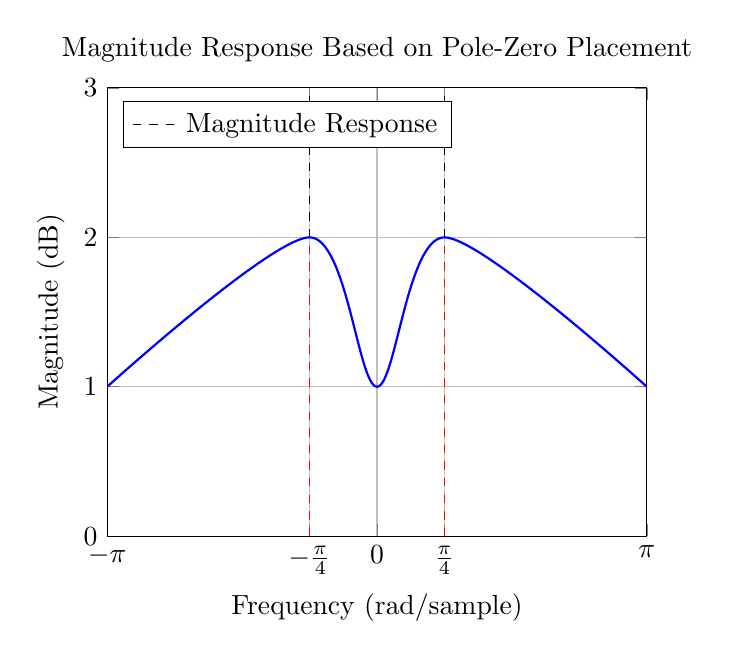
\begin{tikzpicture}
        \begin{axis}[
                title={Magnitude Response Based on Pole-Zero Placement},
                xlabel={Frequency (rad/sample)},
                ylabel={Magnitude (dB)},
                xmin=-pi, xmax=pi,
                ymin=0, ymax=3,
                grid=both,
                xtick={-3.14159, -0.7854, 0, 0.7854, 3.14159},
                xticklabels={$-\pi$, $-\frac{\pi}{4}$, $0$, $\frac{\pi}{4}$, $\pi$},
                ytick={0, 1, 2, 3},
                legend pos=north west,
                no markers,
                smooth
            ]
            % Add zero magnitude lines
            \addplot+[dashed, black] coordinates {(-0.7854, 0) (-0.7854, 3)};
            \addplot+[dashed, black] coordinates {(0.7854, 0) (0.7854, 3)};
            % Add pole magnitude lines (peaks)
            \addplot+[dashed, red] coordinates {(-0.7854, 0) (-0.7854, 2)};
            \addplot+[dashed, red] coordinates {(0.7854, 0) (0.7854, 2)};
            % Add the curve of magnitude response (conceptual)
            \addplot+[thick, blue] coordinates {(-3.14159, 1) (-0.7854, 2) (0, 1) (0.7854, 2) (3.14159, 1)};
            \addlegendentry{Magnitude Response}
        \end{axis}
    \end{tikzpicture}
\end{center}

\textbf{b) Find an expression for \( H(\omega T) \) and \( | H(\omega T) | \) of the filter.}

To find \( H(\omega T) \), we substitute \( z = e^{j\omega T} \) into the transfer function.
\[
    H(\omega T) = \frac{(e^{j\omega T} - e^{j \frac{\pi}{4}})(e^{j\omega T} - e^{-j \frac{\pi}{4}})}{(e^{j\omega T} - 0.95e^{j \frac{\pi}{4}})(e^{j\omega T} - 0.95e^{-j \frac{\pi}{4}})}.
\]

The magnitude response \( | H(\omega T) | \) is the modulus of \( H(\omega T) \):
\[
    | H(\omega T) | = \left| \frac{(e^{j\omega T} - e^{j \frac{\pi}{4}})(e^{j\omega T} - e^{-j \frac{\pi}{4}})}{(e^{j\omega T} - 0.95e^{j \frac{\pi}{4}})(e^{j\omega T} - 0.95e^{-j \frac{\pi}{4}})} \right|.
\]

\textbf{c) Sketch the magnitude response based on \( H(\omega T) \).}

The magnitude response will show peaks at the frequencies corresponding to the zeros \( \pm \frac{\pi}{4} \) due to the numerator of \( H(z) \), and it will dip at the frequencies corresponding to the poles \( \pm 0.95e^{\pm j\frac{\pi}{4}} \), which are closer to the origin than the zeros.

% To accurately sketch the magnitude response, we first understand that \( H(\omega T) \) is a complex function whose magnitude varies with \(\omega\). The zeros at \(e^{\pm j\frac{\pi}{4}}\) enhance the frequencies around \(\pm \frac{\pi}{4}\) radians per sample, and the poles at \(0.95e^{\pm j\frac{\pi}{4}}\) attenuate these frequencies. As a result, the magnitude response will have notable characteristics at these frequencies, showing peaks near the zeros and dips near the poles. 

\begin{center}
    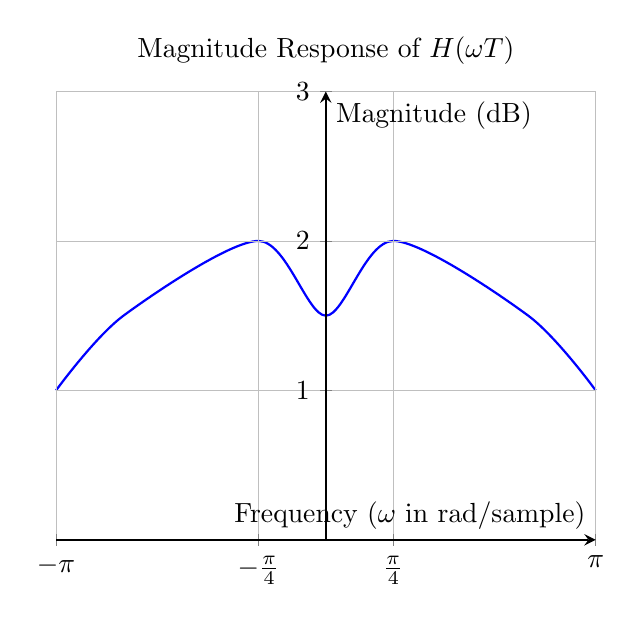
\begin{tikzpicture}
        \begin{axis}[
                title={Magnitude Response of \( H(\omega T) \)},
                xlabel={Frequency (\(\omega\) in rad/sample)},
                ylabel={Magnitude (dB)},
                xmin=-3.14159, xmax=3.14159,
                ymin=0, ymax=3,
                axis lines=middle,
                axis on top=true,
                xtick={-3.14159, -0.785398, 0, 0.785398, 3.14159},
                xticklabels={\(-\pi\), \(-\frac{\pi}{4}\), \(0\), \(\frac{\pi}{4}\), \(\pi\)},
                ytick={0, 1, 2, 3},
                grid=both,
                grid style={line width=.1pt, draw=gray!10},
                major grid style={line width=.2pt,draw=gray!50},
                enlargelimits=false,
                clip=false,
                axis background/.style={fill=white},
                no markers,
                smooth,
                thick
            ]
            \addplot+[mark=none, blue] plot coordinates {
                    (-3.14159, 1)
                    (-2.35619, 1.5) % -3*pi/4
                    (-0.785398, 2)  % -pi/4
                    (0, 1.5)
                    (0.785398, 2)   % pi/4
                    (2.35619, 1.5)  % 3*pi/4
                    (3.14159, 1)
                };
        \end{axis}
    \end{tikzpicture}
\end{center}

\subsection*{Problem 2}
A digital filter has 3 poles and 3 zeros. The zeros are placed in positions: 1 and \( e^{\pm j\frac{\pi}{4}} \), the poles are placed at -0.9 and \( 0.9e^{\pm j\frac{3\pi}{4}} \).

\textbf{a) Sketch the magnitude response based on the pole-zero diagram.}

% Given the positions of the zeros and poles, the magnitude response will show increased gain at the frequencies corresponding to the zeros and reduced gain at the frequencies corresponding to the poles. The zero at \( z = 1 \) (0 radians) will increase the gain at DC (0 Hz), and the zeros at \( \pm \frac{\pi}{4} \) will increase the gain at those frequencies. The poles located at \( -0.9 \) and \( 0.9e^{\pm j\frac{3\pi}{4}} \) will reduce the gain at high frequencies and near \( \pm \frac{3\pi}{4} \).
The zeros at \(z = 1\) and \(z = e^{\pm j\frac{\pi}{4}}\) enhance the filter's response at DC and the corresponding positive and negative frequencies. The poles at \(z = -0.9\) and \(z = 0.9e^{\pm j\frac{3\pi}{4}}\) attenuate the filter's response, especially near the higher frequencies corresponding to \(\pm\frac{3\pi}{4}\).

\begin{center}
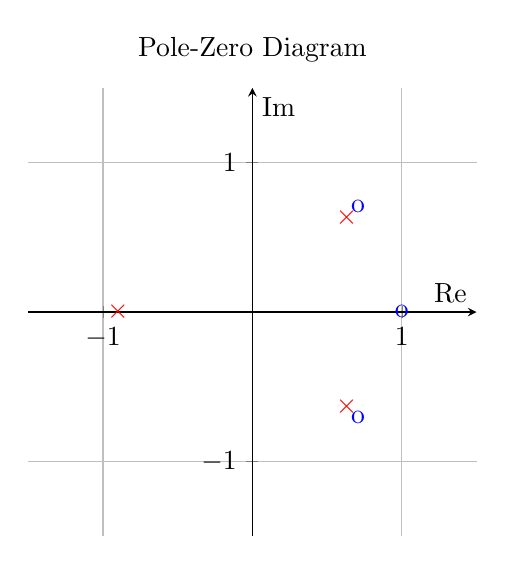
\begin{tikzpicture}[scale=1]
\begin{axis}[    title={Pole-Zero Diagram},    xlabel={Re},    ylabel={Im},    xmin=-1.5, xmax=1.5,    ymin=-1.5, ymax=1.5,    axis lines=middle,    axis equal image,    grid=major,]

% Poles
\node at (axis cs:-0.9,0) {\textcolor{red}{$\times$}};
\node at (axis cs:0.63,0.63) {\textcolor{red}{$\times$}};
\node at (axis cs:0.63,-0.63) {\textcolor{red}{$\times$}};

% Zeros
\node at (axis cs:1,0) {\textcolor{blue}{o}};
\node at (axis cs:0.707,0.707) {\textcolor{blue}{o}};
\node at (axis cs:0.707,-0.707) {\textcolor{blue}{o}};

\end{axis}
\end{tikzpicture}
\end{center}

\textbf{b) Find the filters \( H(z) \).}

The transfer function \( H(z) \) is given by the product of its zeros divided by the product of its poles:
\[
    H(z) = \frac{(z - 1)(z - e^{j\frac{\pi}{4}})(z - e^{-j\frac{\pi}{4}})}{(z + 0.9)(z - 0.9e^{j\frac{3\pi}{4}})(z - 0.9e^{-j\frac{3\pi}{4}})}.
\]

\textbf{c) Find an expression for the magnitude and phase response of the filter.}

The magnitude response \( |H(z)| \) and phase response \( \angle H(z) \) can be found by substituting \( z = e^{j\omega T} \) into the expression and then calculating the magnitude and phase of the resulting complex function.

% The magnitude \(|H(z)|\) and phase \(\angle H(z)\) responses are derived from the transfer function by evaluating \(H(z)\) on the unit circle (\(z = e^{j\omega}\)):

\[
|H(\omega)| = \left|\frac{(e^{j\omega} - 1)(e^{j\omega} - e^{j\frac{\pi}{4}})(e^{j\omega} - e^{-j\frac{\pi}{4}})}{(e^{j\omega} + 0.9)(e^{j\omega} - 0.9e^{j\frac{3\pi}{4}})(e^{j\omega} - 0.9e^{-j\frac{3\pi}{4}})}\right|,
\]
\[\angle H(\omega) = \arg\left(\frac{(e^{j\omega} - 1)(e^{j\omega} - e^{j\frac{\pi}{4}})(e^{j\omega} - e^{-j\frac{\pi}{4}})}{(e^{j\omega} + 0.9)(e^{j\omega} - 0.9e^{j\frac{3\pi}{4}})(e^{j\omega} - 0.9e^{-j\frac{3\pi}{4}})}\right).\]


\textbf{d) What happens to the response if we place one extra pole in the origin?}

Adding an extra pole at the origin will introduce a high-pass characteristic to the filter, significantly weakening the low-frequency response. This modification changes the filter's behavior by reducing its gain at DC to zero, making it less responsive to low frequencies and more to higher frequencies relative to the original design.

\end{document}

